\documentclass[tikz,border=2pt]{standalone}
\usepackage{tikz,amsmath}
\usetikzlibrary{arrows.meta, bending,calc,decorations.markings}
\newcommand{\bmR}{\boldsymbol{\mathcal{R}}}
\begin{document}
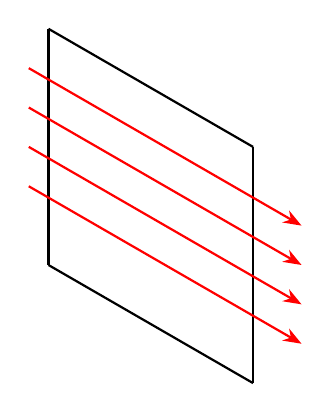
\begin{tikzpicture}[>=Stealth]

% Draw lines and name the endpoints 'A' and 'B'
    \draw [thick] (0.5,2.5) -- ++(-30:3) coordinate (A);
    \draw [thick] (0.5,-0.5) -- ++(-30:3) coordinate (B);
    
    % Draw the start connector
    \draw [thick] (0.5,2.5) -- (0.5,-0.5);
    
    % Draw the end connector using the names
    \draw [thick] (A) -- (B);

\foreach \y in {0, 0.5, 1.0, 1.5} {
        % Start at (0, \y), then move 4 units at a 30-degree angle
        \draw [thick, red,->] (0.25, 0.5+\y) -- ++(-30:4);
    }




\end{tikzpicture}
\end{document}